\documentclass[12pt,twoside]{manual}

 
\newglossaryentry{austenite}
{
    name=austenite,
    description={Austenite is gamma phased iron which has a face centered cubic structure.  May be stabilised with Nickel, Manganese, Copper.}
}

\newglossaryentry{eutectic}
{
    name=eutectic,
    description={A eutectic contains two or more elements, and has a lower melting point than any of it's constituent elements.}
}
 
\newglossaryentry{cubic}
{
    name=cubic,
    description={Cubic: $a = b = c$, $ \alpha = \beta = \gamma = 90^{\circ}$}
}

\newglossaryentry{hexagonal}
{
    name=hexagonal,
    description={Hexagonal: $a = b, c $, $ \alpha = \beta, \gamma = 120^{\circ}$}
}
\newglossaryentry{rhombohedral}
{
    name=rhombohedral,
    description={Rhombohedral: $a = b = c $, $ \alpha = \beta = \gamma \neq 90^{\circ}$}
}
\newglossaryentry{tetragonal}
{
    name=tetragonal,
    description={Tetragonal: $a = b, c $, $ \alpha = \beta = \gamma = 90^{\circ}$}
}
\newglossaryentry{orthorhombic}
{
    name=orthorhombic,
    description={Orthorhombic: $a, b, c $, $ \alpha = \beta = \gamma = 90^{\circ}$}
}
\newglossaryentry{monoclinic}
{
    name=monoclinic,
    description={Monoclinic: $a, b, c $, $ \alpha = \beta = 90, \gamma \neq 90^{\circ}$}
}
\newglossaryentry{triclinic}
{
    name=triclinic,
    description={Triclinic: $a, b, c $, $ \alpha, \beta, \gamma, $}
}





\newacronym{gif}{GIF}{Generation IV International Forum}
\newacronym{geniv}{GenIV}{Generation IV}



\newacronym{pwr}{PWR}{Pressurised Water Reactor}
\newacronym{lwr}{LWR}{Light Water Reactor}
\newacronym{bwr}{BWR}{Boiling Water Reactor}
\newacronym{agr}{AGR}{Advanced Gas Reactor}
\newacronym{epr}{EPR}{European Pressurised Reactor}
\newacronym{abwr}{ABWR}{Advanced Boiling Water Reactor}
\newacronym{gfr}{GFR}{Gas-Cooled Fast Reactor}
\newacronym{lfr}{LFR}{Lead-Cooled Fast Reactor}
\newacronym{msr}{MSR}{Molten Salt Reactor}
\newacronym{scwr}{SCWR}{Supercritical-Water-Cooled Reactor}
\newacronym{sfr}{SFR}{Sodium-Cooled Fast Reactor}
\newacronym{vhtr}{VHTR}{Very-High-Temperature Reactor}
\newacronym{fnr}{FNR}{Fast-Neutron Reactors}
\newacronym{elsy}{ELSY}{European Lead Fast Reactor}
\newacronym{fbr}{FBR}{Fast Breeder Reactor}
\newacronym{pbr}{FBR}{Pebble-Bed Reactor}
\newacronym{npp}{NPP}{Nuclear Power Plant}


\newacronym{triso}{TRISO}{Tristructural Isotropic}

\newacronym{ccgt}{CCGT}{Combined Cycle Gas Turbine}


\newacronym{endf}{ENDF}{Evaluated Nuclear Data File}
\newacronym{nea}{NEA}{Nuclear Energy Agency}
\newacronym{jeff}{JEFF}{Joint Evaluated Fission and Fusion File}



\newacronym{sc}{SC}{Simple Cubic}
\newacronym{bcc}{BCC}{Body Centered Cubic}
\newacronym{fcc}{FCC}{Face Centered Cubic}
\newacronym{fct}{FCT}{Face Centered Tetragonal}
\newacronym{zb}{ZB}{Zinc Blende}

\newacronym{hrb}{HRB}{Hardness Rockwell B}


\newacronym{md}{MD}{Molecular Dynamics}
\newacronym{eam}{EAM}{Embedded-Atom method}

\newacronym{hf}{HF}{Hartree-Fock}

\newacronym{dft}{DFT}{Density Functional Theory}
\newacronym{scf}{SCF}{Self Consistent Field}
\newacronym{pbe}{PBE}{Perdew-Burke-Ernzerhof}
\newacronym{pz}{PZ}{Perdew-Zunger}
\newacronym{lda}{LDA}{Local Density Approximation}
\newacronym{gga}{GGA}{Generalized Gradient Approximation}
\newacronym{zbl}{ZBL}{Ziegler-Biersack-Littmark}

\newacronym{igscc}{IGSCC}{Intergranular Stress Corrosion Cracking}
\newacronym{iascc}{IASCC}{Irradiation Assisted Stress Corrosion Cracking}
\newacronym{scc}{SCC}{Stress Corrosion Cracking}
\newacronym{ris}{RIS}{Radiation Induced Segregation}
\newacronym{rip}{RIP}{Radiation Induced Precipitation}

\newacronym{dpa}{DPA}{Displacements Per Atom}
\newacronym{vpi}{VPI}{Vacancies Per Ion}
\newacronym{pka}{PKA}{Primary Knock-On Atom}


\newacronym{edf}{EDF}{Électricité de France}




\newacronym{ornl}{ORNL}{Oak Ridge National Laboratory}
\newacronym{linac}{LINAC}{Linear Accelerator}
\newacronym{sns}{SNS}{Spallation Neutron Source}
\newacronym{rfq}{RFQ}{Radio Frequency Quadrupole}
\newacronym{hfir}{HFIR}{High Flux Isotope Reactor}




\newacronym{srim}{SRIM}{Stopping Range In Matter}
\newacronym{trim}{TRIM}{Transport In Matter}



\makeglossaries


\include{tikz}

\usepackage{listings}
\lstloadlanguages{Fortran,Bash,Python,C++}
\lstloadlanguages{Matlab}

\lstdefinestyle{inputfile}
{
  breaklines=true,
  numbers=left,
  stepnumber=1,
  tabsize=4,
  numberstyle=\tiny\color{gray},
  keywordstyle=\color{blue},
  commentstyle=\color{dkgreen},
  stringstyle=\color{mauve}
}

\lstdefinestyle{spython}
{
	language=Python,
  breaklines=true,
  numbers=left,
  stepnumber=1,
  tabsize=4,
  numberstyle=\tiny\color{gray},
  keywordstyle=\color{blue},
  commentstyle=\color{dkgreen},
  stringstyle=\color{mauve}
}

\lstdefinestyle{pseudocode}
{
  breaklines=true,
  numbers=left,
  stepnumber=1,
  tabsize=4,
  keywordstyle=\color{blue}
}



\definecolor{col_336699}{RGB}{51,102,153}
\definecolor{col_333333}{RGB}{51,51,51}
\definecolor{col_111111}{RGB}{17,17,17}
\definecolor{col_555555}{RGB}{85,85,85}
\definecolor{col_666666}{RGB}{102,102,102}
\definecolor{col_777777}{RGB}{119,119,119}
\definecolor{col_000022}{RGB}{0,0,34}
\definecolor{col_000000}{RGB}{0,0,0}


 
%% DRAW LINE
\newcommand{\tikzdrawline}[7]{
\draw[#1] (#2,#4,#3) -- (#5,#7,#6);  
}
%% DRAW BALL
\newcommand{\tikzdrawatom}[5]{%
\filldraw[ball color=#1] (#2,#3,#4) circle[radius=#5];
}  

%% DRAW ARROW
\newcommand{\tikzdrawarrow}[9]{
\draw[#1, thick, ->] (#2,#4,#3) -- (#5,#7,#6) node[midway,#8]{#9};  
}

\newcommand{\tikzdrawlinethick}[7]{
\draw[#1, line width=0.5mm] (#2,#4,#3) -- (#5,#7,#6);  
} 

\newcommand{\tikzdrawlinedotted}[7]{
\draw[#1, dotted] (#2,#4,#3) -- (#5,#7,#6);  
}

%% DRAW COORD GRID
\newcommand{\tikzcoordgrid}[6]{%
\fill[col_336699!10,opacity=1.0] (0.0,0.0,0.0) -- (0.0,0.0,#1) -- (0.0,#3,#1) -- (0.0,#3,0.0) -- cycle;
\fill[col_336699!15,opacity=1.0] (0.0,0.0,0.0) -- (0.0,#3,0.0) -- (#2,#3,0.0) -- (#2,0.0,0.0) -- cycle;
\fill[col_336699!30,opacity=1.0] (0.0,0.0,0.0) -- (#2,0.0,0.0) -- (#2,0.0,#1) -- (0.0,0.0,#1) -- cycle;
\tikzdrawarrow{col_000000}{0.0}{0.0}{0.0}{0.0}{1.05*#1}{0.0}{above}{#4};
\tikzdrawarrow{col_000000}{0.0}{0.0}{0.0}{1.05*#1}{0.0}{0.0}{above}{#5};
\tikzdrawarrow{col_000000}{0.0}{0.0}{0.0}{0.0}{0.0}{1.05*#1}{left}{#6};
}  







\pagestyle{plain}
\begin{document}


%%######################################################################
%% Cover Page
%%######################################################################

\begin{titlepage}
  \begin{center}
    \centerline{
\includegraphics[width=0.7\textwidth]{img/coverart}}


    \textbf{Department of Metallurgy \& Materials}

    \vspace*{2.0cm}
    \Large{}
    \textbf{QEEoS Manual}
    \textbf{Equation of State Calculator for Quantum Espresso}
    \vspace{0.8cm}
    \normalsize{}

  \end{center}
\end{titlepage}

\pagenumbering{gobble}

\pagenumbering{roman} 

\tableofcontents

\pagenumbering{arabic}







%%######################################################################
%% Introduction
%%######################################################################

\chapter{Introduction}

\section{What does it do?}

This python code calculates the equation of state and elastic constants of a material.  It prepares input files for Quantum Espresso\cite{quantumespresso}, runs quantum espresso and collects the data.  It calculates the properties and plots the results for the user.  There is an option to cache input/output files such that calculations that have already run aren't repeated.


\section{Download Source Code}

The source code and examples are available to download from github:

https://github.com/BenPalmer1983/qeeos

Quantum Espresso is available to download from their website:

https://www.quantum-espresso.org/download



\section{Requirements}

\begin{itemize}
\item ideally a multicore computer or cluster
\item quantum espresso installed
\item ubuntu or similar operating system
\item python3
\item matplotlib
\end{itemize}



\section{How To Use}

\subsection{Input Files}

An example set of input files is given in the appendix.



\subsection{PWscf Script}

The PWscf program may either be executed using the binary file directly (pw.x) or using a bash script.  During testing, a node with a moderate scratch directory was filling up after every couple of PWscf jobs.  This script creates a log, clears the scratch directory completely and runs PWscf.

\begin{lstlisting}[style=inputfile,caption={PWscf Script}]
#!/bin/bash
touch bash.log
timestamp=$(date +%s)

echo "=============================================================================" >> bash.log
echo "              START                                 " >> bash.log
echo $timestamp >> bash.log
echo "=============================================================================" >> bash.log

echo $OMP_NUM_THREADS >> bash.log
echo $PROC_COUNT >> bash.log
echo $PWSCF_SCRATCH >> bash.log
echo $PWSCF_PP >> bash.log
echo $PWSCF_CACHE >> bash.log
echo $PWSCF_BIN >> bash.log
echo $PWSCF_SCRIPT >> bash.log

rm -R $PWSCF_SCRATCH/*

echo "" >> bash.log
df -h >> bash.log
lscpu >> bash.log
free -h >> bash.log
echo "=============================================================================" >> bash.log
echo $1 >> bash.log
echo $2 >> bash.log
echo $3 >> bash.log
echo "=============================================================================" >> bash.log
echo "              RUNNING                                 " >> bash.log
mpirun -n $1 $PWSCF_BIN -in $2  > $3 
echo "=============================================================================" >> bash.log
df -h >> bash.log
echo "=============================================================================" >> bash.log
echo "              END                                 " >> bash.log
echo $timestamp >> bash.log
echo "=============================================================================" >> bash.log
echo "" >> bash.log
echo "" >> bash.log
echo "" >> bash.log
echo "" >> bash.log
echo "" >> bash.log
echo "" >> bash.log
echo "" >> bash.log
echo "" >> bash.log
echo "" >> bash.log
echo "" >> bash.log
echo "" >> bash.log
\end{lstlisting}


\subsection{PWscf Cache}

A cache directory may be set.  All the output files will be cached, and any repeat input files will be loaded from the cache to eliminate duplicate calculations.


\begin{appendices}


\chapter{Aluminium}

\section{Input Files}

\begin{lstlisting}[style=inputfile,caption={Job Bash Script}]
#!/bin/bash

# Set the number of threads to 1
export OMP_NUM_THREADS=1
export PROC_COUNT=1
export PWSCF_SCRATCH=/opt/scratch
export PWSCF_PP=/opt/pp
export PWSCF_CACHE=/opt/pwscf_cache
export PWSCF_BIN=/opt/qe/bin/pw.x
export PWSCF_SCRIPT=/opt/qe/bin/pw.sh

thisdir=$(pwd)
echo $thisdir
cd ../../
qeeos=$(pwd)
echo $qeeos
./package.sh
cd $thisdir
cp ../../qeeos.py qeeos.py

python3 qeeos.py input.in all
\end{lstlisting}




\begin{lstlisting}[style=inputfile,caption={QEEoS Input File}]
# The template pwscf file
pwscf_template file=alfcc.in

# Crystal
config type=fcc size=2 alat=6.9

# Use almost complete output files
job_done setting=almost

# Convergence settings
settings ecutwfc=50 ecutrho=200 kpoints='11 11 11 1 1 1' kpointstype='automatic' degauss=0.04

# EoS and EC strain and point count
eos points=11 strain=0.005
ec points=9 strain=0.005
\end{lstlisting}



\begin{lstlisting}[style=inputfile,caption={PWscf file - template}]
! Aluminium Input File
&CONTROL 
calculation = "scf", 
disk_io = 'low', 
etot_conv_thr = 1.0E-4, 
forc_conv_thr = 1.0D-3, 
nstep = 50, 
outdir = "/opt/scratch", 
prefix = "fe_scf_fcc_2", 
pseudo_dir = "/opt/pp", 
restart_mode = 'from_scratch', 
tprnfor = .true., 
tstress = .true., 
/ 
&SYSTEM 
celldm(1) = 7.5, 
ecutrho = 200, 
ecutwfc = 50, 
ibrav = 0, 
nat = 4, 
ntyp = 1, 
nspin = 1,
starting_magnetization(1) = 0,
occupations = 'smearing',
smearing = 'mv',
degauss = 0.02,
/ 
&ELECTRONS 
conv_thr = 1.0D-6, 
diagonalization = 'david', 
mixing_beta = 1.0000000E-01, 
mixing_mode = 'plain', 
mixing_ndim = 10, 
/ 
&IONS 
ion_dynamics = 'bfgs', 
/ 
&CELL 
cell_dynamics = 'bfgs', 
cell_factor = 2.0, 
press = 0.0, 
/ 
ATOMIC_SPECIES 
Al 26.982 Al.pbe-nl-kjpaw_psl.1.0.0.UPF 
ATOMIC_POSITIONS crystal
Al   0.0   0.0   0.0   
Al   0.5   0.5   0.0   
Al   0.5   0.0   0.5   
Al   0.0   0.5   0.5   
K_POINTS automatic
5 5 5   1 1 1 
CELL_PARAMETERS alat
1.0 0.0 0.0 
0.0 1.0 0.0 
0.0 0.0 1.0
\end{lstlisting}


\begin{lstlisting}[style=inputfile,caption={Run Command}]
./run.sh
\end{lstlisting}




\section{Results}

\subsection{Plots}

\FloatBarrier

\begin{figure}[htbp]
  \begin{center}
    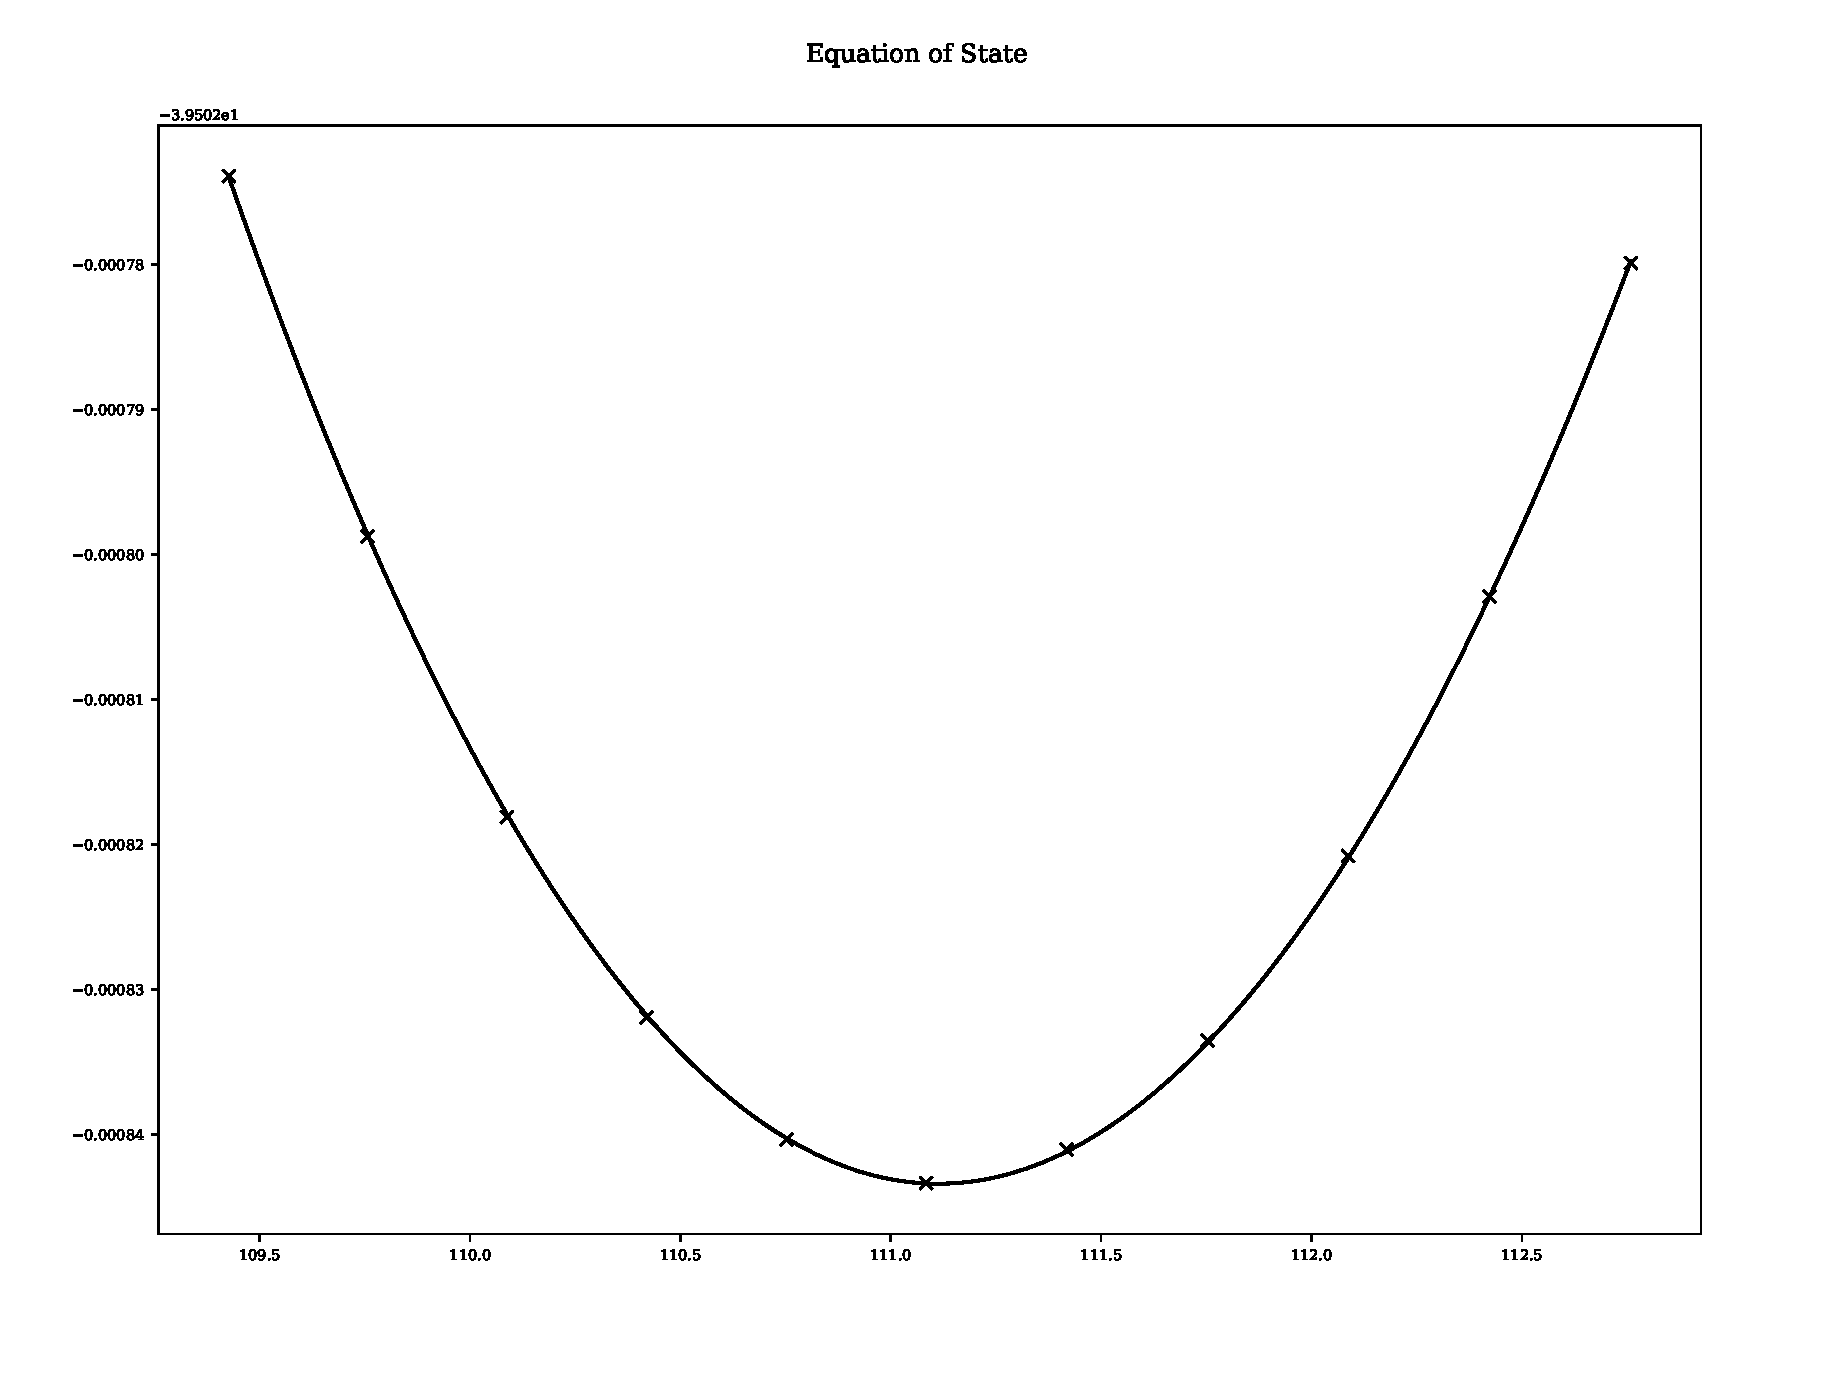
\includegraphics[width=15.0cm]{img/aleos.eps}
    \captionsetup{font={it}}
    \caption{Aluminium Equation of State Plot}
    \label{fig:aleos}
  \end{center}
\end{figure}

\begin{figure}[htbp]
  \begin{center}
    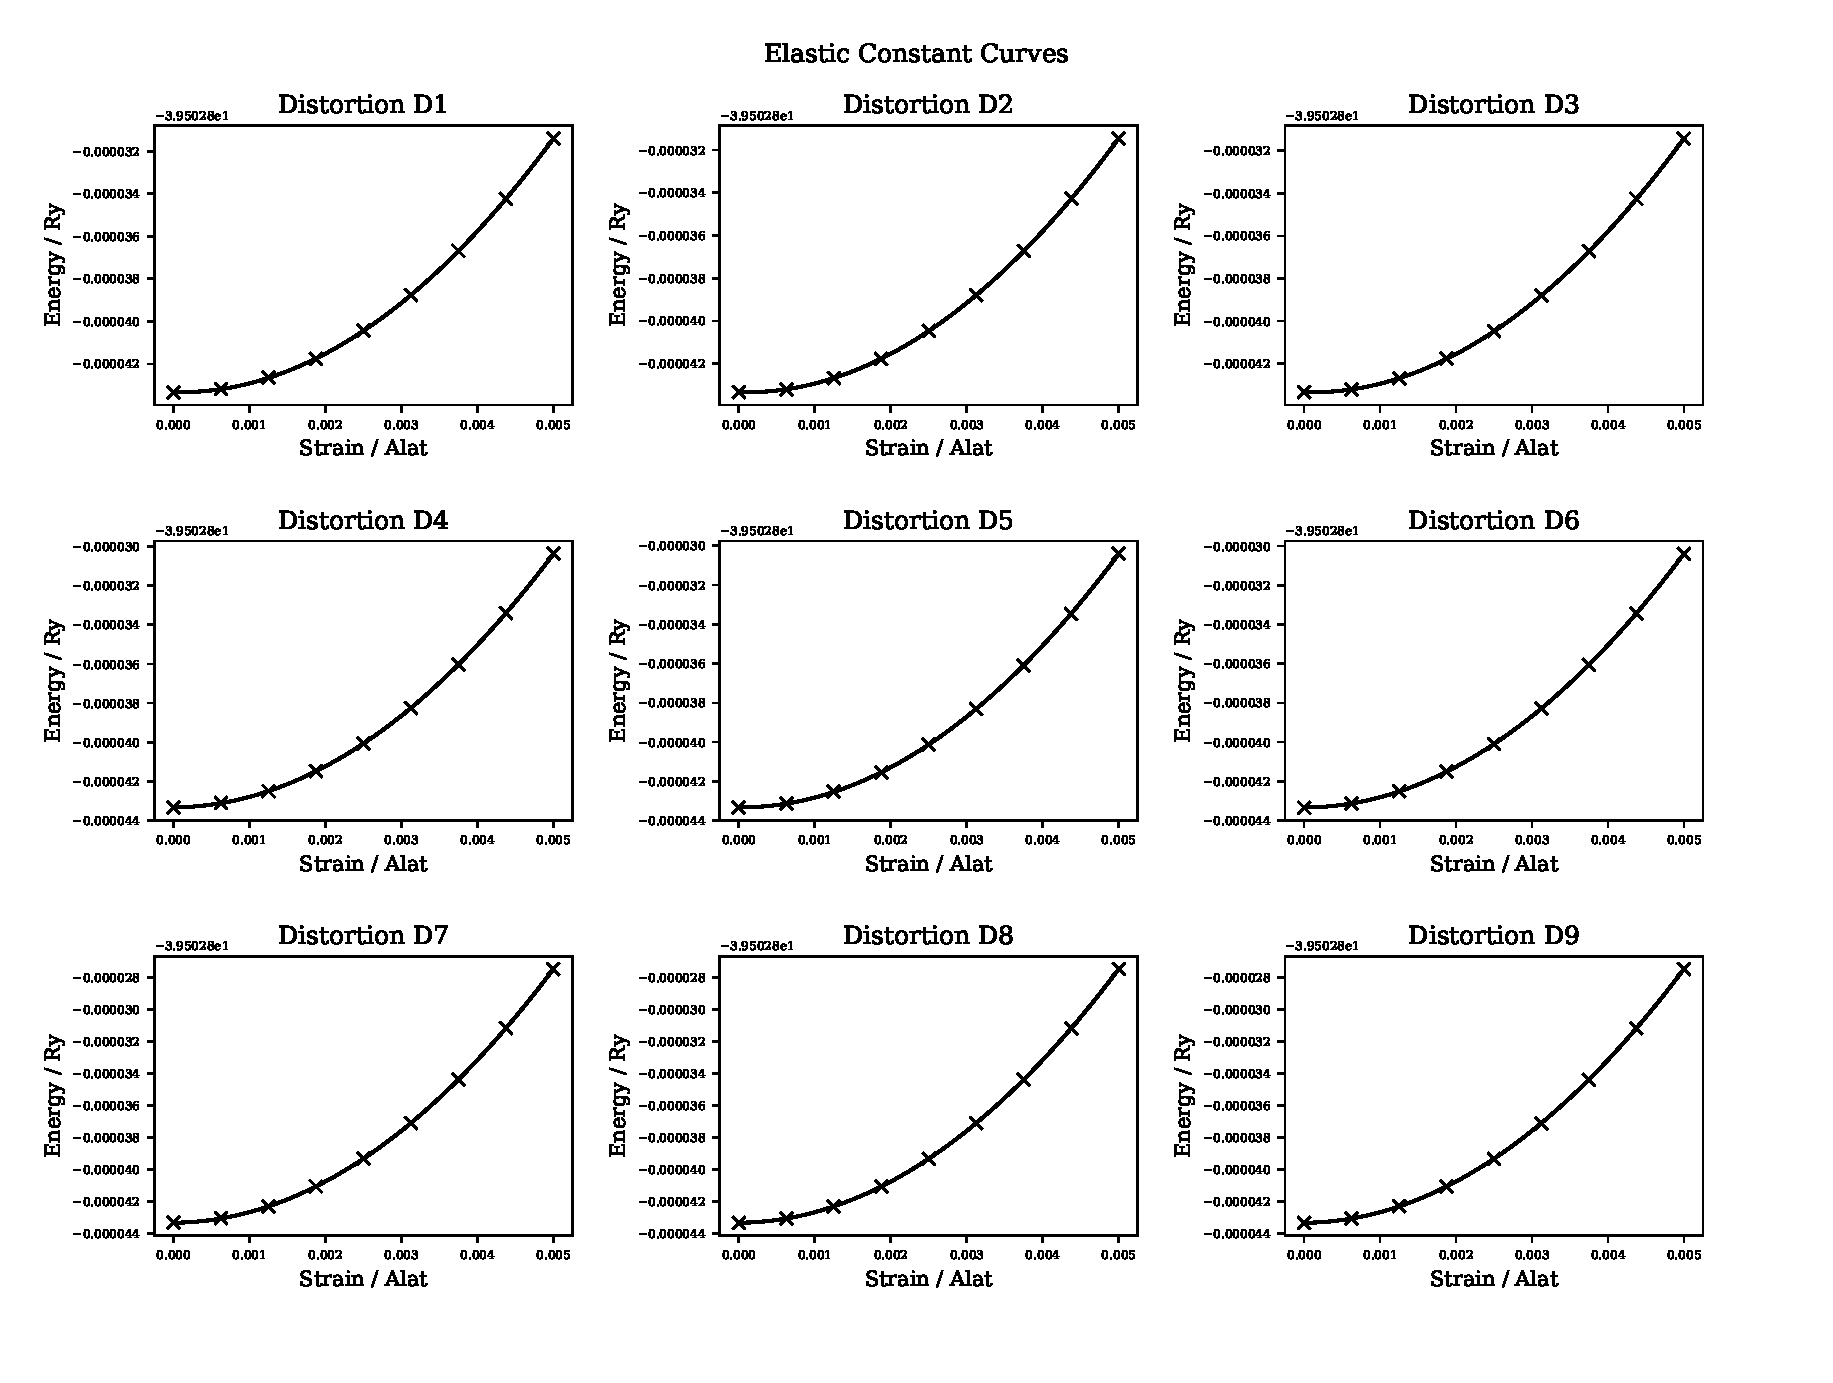
\includegraphics[width=15.0cm]{img/alec.eps}
    \captionsetup{font={it}}
    \caption{Aluminium Elastic Constant Distortions}
    \label{fig:alec}
  \end{center}
\end{figure}

\FloatBarrier

\subsection{Calculated Properties}

\begin{lstlisting}[style=inputfile,caption={Results File}]
################################################################
#                        RESULTS                               #
################################################################
Fri, 14 May 2021 12:36:52 +0000

INPUT SETTINGS
################################

Structure:                    None
Size:                         2
A0:                           6.9
A0 Units:                     angs
A0 (Bohr):                    7.5
A0 (Angs):                    3.9675000000000002

Ecutwfc:                      50
Ecutrho:                      200
Degauss:                      0.04
Kpoints:                      11 11 11 1 1 1
Kpoints Type:                 automatic
EOS Points:                   11
EOS Strain:                   0.005
EC Points:                    9
EC Strain:                    0.005


RELAXED
################################

a0 (Bohr):                    7.630815
CP:                           1.0      0.0      0.0
                              0.0      1.0      0.0
                              0.0      0.0      1.0
Volume (Bohr^3/unit cell):    444.337302525
Density KG/m^3:               2724.60378074
AMU per crystal unit:         107.928
Atoms per crystal unit:       4
Total Energy/Ry:              -158.01137346
Energy per Atom/Ry:           -39.502843365
Total Force Ry/Bohr:          0.0
Force per atom Ry/Bohr:       0.0


a0 primitive (Bohr):          3.8154075
a0 primitive (Ang):          2.0183505675


EOS
################################

V0 (Bohr^3 / atom):           111.113040914
E0 (Ry / atom):               -39.5028433791
B0 (RY/BOHR3):                0.00532062822795
B0 (GPA):                     78.2691015472
B0P:                          1.1603824335


EC
################################

Stiffness (RY/BOHR3):         0.0088737  0.0032167  0.0032394  0.0        0.0        0.0       
                              0.0032167  0.0088603  0.0032408  0.0        0.0        0.0       
                              0.0032394  0.0032408  0.0089149  0.0        0.0        0.0       
                              0.0        0.0        0.0        0.0023131  0.0        0.0       
                              0.0        0.0        0.0        0.0        0.0023436  0.0       
                              0.0        0.0        0.0        0.0        0.0        0.0023259 

Stiffness (GPA):              129.410255 46.9113771 47.2423723 0.0        0.0        0.0       
                              46.9113771 129.215660 47.2632875 0.0        0.0        0.0       
                              47.2423723 47.2632875 130.012231 0.0        0.0        0.0       
                              0.0        0.0        0.0        33.7329257 0.0        0.0       
                              0.0        0.0        0.0        0.0        34.1775875 0.0       
                              0.0        0.0        0.0        0.0        0.0        33.9197927

Compliance (1/GPA):           0.0095831  -0.0025437 -0.0025575 0.0        0.0        0.0       
                              -0.0025437 0.009601   -0.002566  0.0        0.0        0.0       
                              -0.0025575 -0.002566  0.0095537  0.0        0.0        0.0       
                              0.0        0.0        0.0        0.0296446  0.0        0.0       
                              0.0        0.0        0.0        0.0        0.0292589  0.0       
                              0.0        0.0        0.0        0.0        0.0        0.0294813 

Stability:
C11:                                                129.410255755 (Stable)
C11C22 - C12C12:                                    14521.1543769 (Stable)
C11*C22*C33+2*C12*C13*C23-C11*C23*C23-C33*C12*C12:  1808338.92098 (Stable)
C44:                                                33.732925686 (Stable)
C55:                                                34.177587473 (Stable)
C66:                                                33.919792695 (Stable)

Bulk Modulus B (GPA):         74.6075275525
BR (GPA):                     74.6070305059
BV (GPA):                     74.6080245991

Shear Modulus G (GPA):        36.6819340254
GR:                           36.5163995062
GV:                           36.8474685447

Young's Modulus E (GPA):      94.5501288998

Poisson's Ratio v:            0.288783312709


L Elastic Wave V:             0.212917466944
T Elastic Wave V:             0.116031106888
M Elastic Wave V:             0.129421644875

Debye Temperature:            0.00151522447134

Melting Point:                1410.0K 


References 
=======================================

First Principles Calculations of Elastic Properties of Metals
M. J. Mehl, B. M. Klein, D. A. Papaconstantopoulos
1994

Ab Initio Study of the Elastic and Mechanical Properties of B19 TiAl
Y. Wen, L. Wang, H. Liu and L. Song
Crystals
2017

Density functional theory for calculation of elastic properties of orthorhombic crystals - applications to TiSi2
P. Ravindran, Lars Fast, P. A. Korzhavyi, B. Johansson
Journal of Applied Physics
1998
\end{lstlisting}





\chapter{BCC Iron}

\section{Input Files}


\begin{lstlisting}[style=inputfile,caption={Job Bash Script}]
#!/bin/bash

# Set the number of threads to 1
export OMP_NUM_THREADS=1
export PROC_COUNT=16
export PWSCF_SCRATCH=/opt/scratch
export PWSCF_PP=/opt/pp
export PWSCF_CACHE=/opt/pwscf_cache
export PWSCF_BIN=/opt/qe/bin/pw.x
export PWSCF_SCRIPT=/opt/qe/bin/pw.sh

thisdir=$(pwd)
echo $thisdir
cd ../../
qeeos=$(pwd)
echo $qeeos
./package.sh
cd $thisdir
cp ../../qeeos.py qeeos.py

python3 qeeos.py input.in all
\end{lstlisting}


\begin{lstlisting}[style=inputfile,caption={Job SBATCH Script}]
#!/bin/bash
#
#SBATCH --job-name=pwfeeosbccmag
#SBATCH --output=jobout.txt
#SBATCH --account=readmsd02
#
#SBATCH --ntasks 40
#SBATCH --nodes 1
#SBATCH --time 1200:00
#SBATCH --mem 120GB
#
#SBATCH --get-user-env
#SBATCH --export=NONE
#
unset SLURM_EXPORT_ENV

#module purge; module load bluebear
#module load bear-apps/2018a
#module load imkl 2019.5.281-gompi-2019b
#module load Python 3.7.4-GCCcore-8.3.0
#module load matplotlib 3.1.1-foss-2019b-Python-3.7.4

module purge; module load bluebear
module load bear-apps/2018a
module load iomkl/2018a
module load Python/3.6.3-iomkl-2018a
module load matplotlib/2.1.1-iomkl-2018a-Python-3.6.3

# Change to $PBS_O_WORKDIR
cd "$PBS_O_WORKDIR"
# Set the number of threads to 1
export OMP_NUM_THREADS=1
export PROC_COUNT=40
export PWSCF_SCRATCH=/scratch
export PWSCF_PP=/rds/homes/b/bxp912/pp
export PWSCF_CACHE=/rds/homes/b/bxp912/pwscf_cache
export PWSCF_BIN=/rds/homes/b/bxp912/apps/qe-6.3/bin/pw.x
export PWSCF_SCRIPT=/rds/homes/b/bxp912/apps/qe-6.3/bin/pw.sh

python /rds/homes/b/bxp912/apps/python/qeeos.py input.in > result.txt
\end{lstlisting}







\begin{lstlisting}[style=inputfile,caption={QEEoS Input File}]
# The template pwscf file
pwscf_template file=febcc.in
settings ecutwfc=71 ecutrho=430 kpoints='9 9 9 1 1 1' kpointstype='automatic' degauss=0.04 

config structure=bcc size=2 alat=2.8 alat_units=ang
job_done setting=almost

ec run=true points=7 strain=0.004
eos run=true points=15 strain=0.02

\end{lstlisting}



\begin{lstlisting}[style=inputfile,caption={PWscf file - template}]
! Edited 18:37   5/12/2018
&CONTROL 
calculation = "scf", 
disk_io = 'low', 
etot_conv_thr = 1.0E-4, 
forc_conv_thr = 1.0D-3, 
nstep = 40, 
outdir = "/opt/scratch", 
prefix = "fe_fcc_1", 
pseudo_dir = "/opt/pp", 
restart_mode = 'from_scratch', 
tprnfor = .true., 
tstress = .true., 
/ 
&SYSTEM 
celldm(1) = 7.5, 
ecutrho = 200, 
ecutwfc = 35, 
ibrav = 0, 
nat = 4, 
ntyp = 2, 
nspin = 2,
starting_magnetization(1) = 0.1,
starting_magnetization(2) = 0.1,
occupations = 'smearing',
smearing = 'mv',
degauss = 0.05,
/ 
&ELECTRONS 
conv_thr = 1.0D-6, 
diagonalization = 'david', 
mixing_beta = 1.0000000E-01, 
mixing_mode = 'plain', 
mixing_ndim = 10, 
/ 
&IONS 
ion_dynamics = 'bfgs', 
/ 
&CELL 
cell_dynamics = 'bfgs', 
cell_factor = 2.0, 
press = 0.0, 
/ 
ATOMIC_SPECIES 
Fe1   55.845   Fe.pbe-spn-kjpaw_psl.1.0.0.UPF
Fe2   55.845   Fe.pbe-spn-kjpaw_psl.1.0.0.UPF
ATOMIC_POSITIONS crystal
Fe1   0.0   0.0   0.0   
Fe2   0.5   0.5   0.0   
K_POINTS automatic
5 5 5   1 1 1 
CELL_PARAMETERS alat
1.0 0.0 0.0 
0.0 1.0 0.0 
0.0 0.0 1.0
\end{lstlisting}


\begin{lstlisting}[style=inputfile,caption={Run Command}]
./run.sh
\end{lstlisting}




\section{Results}

\subsection{Plots}

\FloatBarrier
\begin{figure}[htbp]
  \begin{center}
    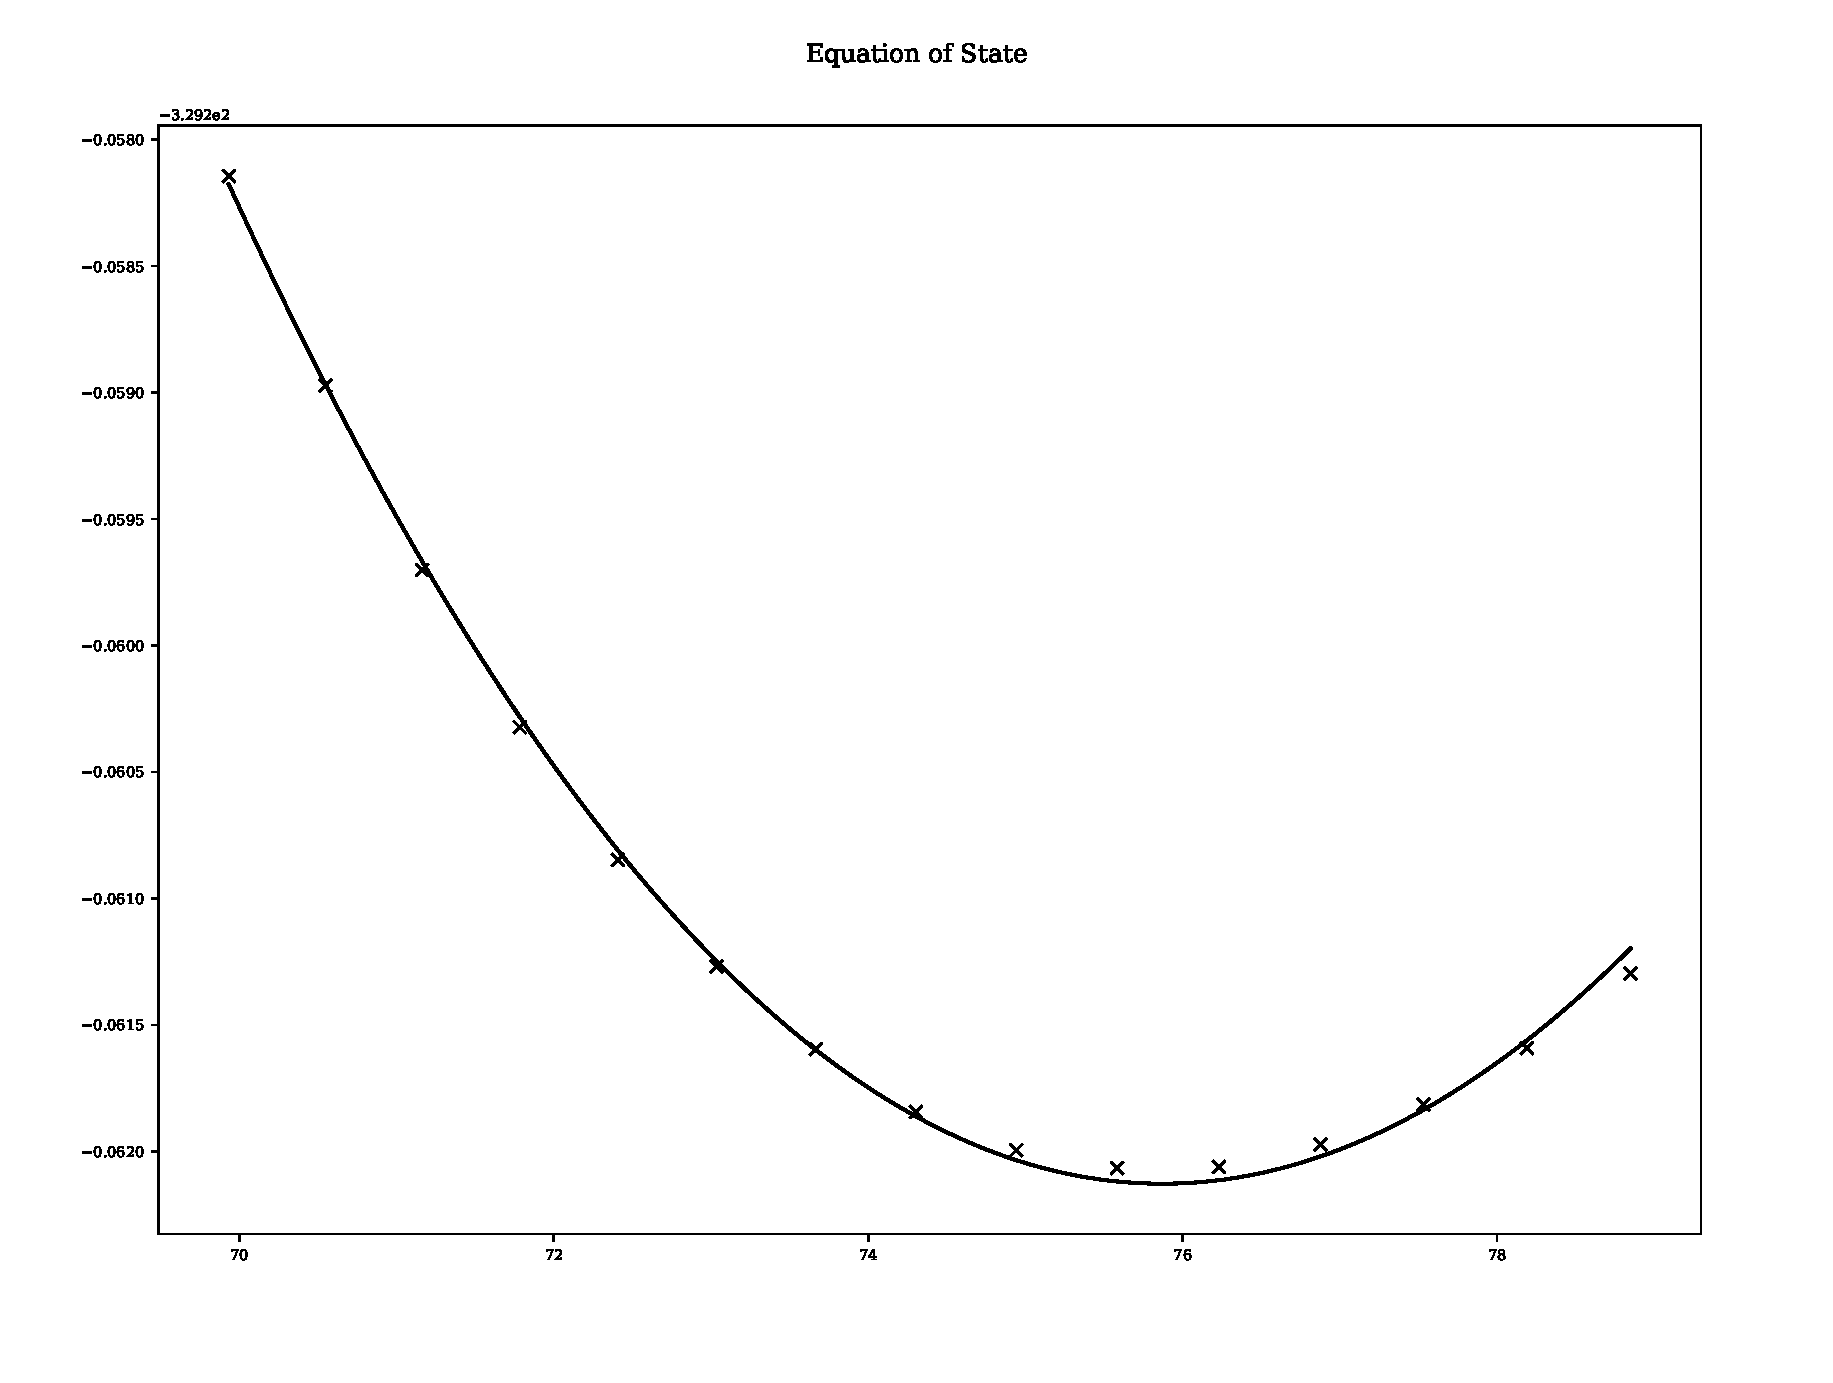
\includegraphics[width=15.0cm]{img/feeos.eps}
    \captionsetup{font={it}}
    \caption{Iron Equation of State Plot}
    \label{fig:feeos}
  \end{center}
\end{figure}

\begin{figure}[htbp]
  \begin{center}
    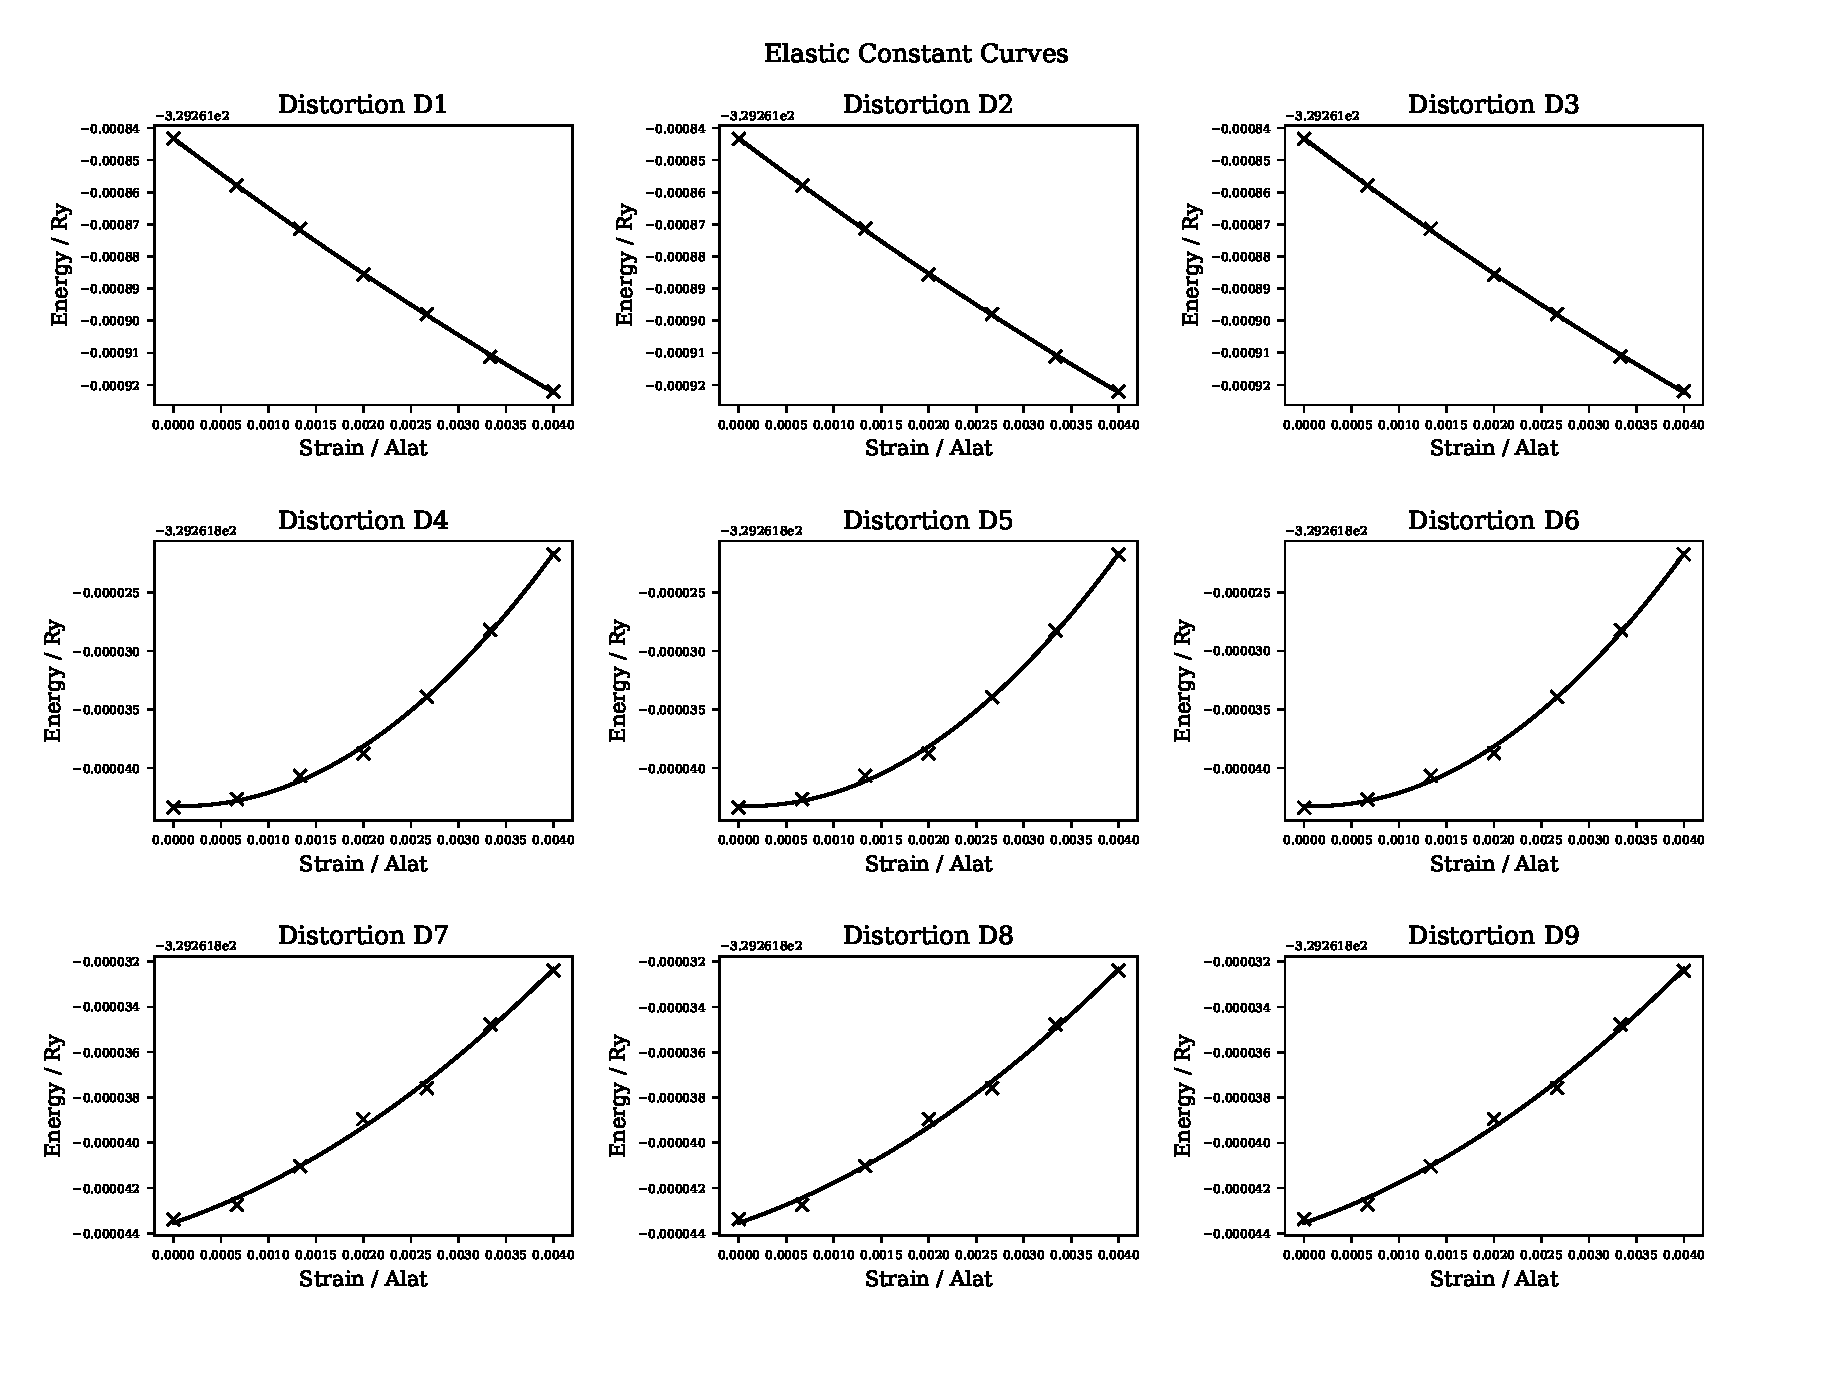
\includegraphics[width=15.0cm]{img/feec.eps}
    \captionsetup{font={it}}
    \caption{Iron Elastic Constant Distortions}
    \label{fig:feec}
  \end{center}
\end{figure}
\FloatBarrier

\subsection{Calculated Properties}

\begin{lstlisting}[style=inputfile,caption={Results File}]
################################################################
#                        RESULTS                               #
################################################################
Tue, 03 Nov 2020 00:43:59 +0000

INPUT SETTINGS
################################

Structure:                    bcc
Size:                         2
Alat:                         2.8
Alat Units:                   ang
A0/Bohr:                      10.584
A0/Bohr Primitive:            5.292
A0/Ang:                       5.599
A0/Ang Primitive:             2.799

Ecutwfc:                      71
Ecutrho:                      430
Degauss:                      0.04
Kpoints:                      9 9 9 1 1 1
Kpoints Type:                 automatic
EOS Points:                   15
EOS Strain:                   0.02
EC Points:                    7
EC Strain:                    0.004


RELAXED
################################

a0 (Bohr):                    10.5935195777
CP:                           1.0      0.0      0.0
                              0.0      1.0      0.0
                              0.0      0.0      1.0
Volume (Bohr^3/unit cell):    1188.83291445
Density KG/m^3:               8430.73536197
AMU per crystal unit:         893.5200000000003
Atoms per crystal unit:       16
Total Energy/Ry:              -5268.18846365
Energy per Atom/Ry:           -329.261778978125
Total Force Ry/Bohr:          2.2e-05
Force per atom Ry/Bohr:       1.375e-06


EOS
################################

V0 (Bohr^3 / atom):           75.8702665574
E0 (Ry / atom):               -329.262127846
B0 (RY/BOHR3):                0.0162627705049
B0 (GPA):                     239.233485512
B0P:                          3.31889213904


EC
################################

Stiffness (RY/BOHR3):         0.0171516  0.0124976  0.0125676  0.0        0.0        0.0       
                              0.0124976  0.0170822  0.0125444  0.0        0.0        0.0       
                              0.0125676  0.0125444  0.0172259  0.0        0.0        0.0       
                              0.0        0.0        0.0        0.0095442  0.0        0.0       
                              0.0        0.0        0.0        0.0        0.0095793  0.0       
                              0.0        0.0        0.0        0.0        0.0        0.0095537 

Stiffness (GPA):              250.132342 182.259746 183.281637 0.0        0.0        0.0       
                              182.259746 249.120299 182.943193 0.0        0.0        0.0       
                              183.281637 182.943193 251.216666 0.0        0.0        0.0       
                              0.0        0.0        0.0        139.188773 0.0        0.0       
                              0.0        0.0        0.0        0.0        139.701369 0.0       
                              0.0        0.0        0.0        0.0        0.0        139.328420

Compliance (1/GPA):           0.0104302  -0.0043908 -0.0044121 0.0        0.0        0.0       
                              -0.0043908 0.0104768  -0.0044261 0.0        0.0        0.0       
                              -0.0044121 -0.0044261 0.0104228  0.0        0.0        0.0       
                              0.0        0.0        0.0        0.0071845  0.0        0.0       
                              0.0        0.0        0.0        0.0        0.0071581  0.0       
                              0.0        0.0        0.0        0.0        0.0        0.0071773 

Stability:
C11:                                                250.132342608 (Stable)
C11C22 - C12C12:                                    29094.4289627 (Stable)
C11*C22*C33+2*C12*C13*C23-C11*C23*C23-C33*C12*C12:  11159908.42 (Stable)
C44:                                                139.188773945 (Stable)
C55:                                                139.701369768 (Stable)
C66:                                                139.328420919 (Stable)

Bulk Modulus B (GPA):         205.266898691
BR (GPA):                     205.262857117
BV (GPA):                     205.270940264

Shear Modulus G (GPA):        79.444946448
GR:                           61.7805312161
GV:                           97.10936168

Young's Modulus E (GPA):      211.100582284

Poisson's Ratio v:            0.328596668021


L Elastic Wave V:             0.192124400694
T Elastic Wave V:             0.0970734376997
M Elastic Wave V:             0.108830260592

Debye Temperature:            0.000728462246711

Melting Point:                2076.0K 








References 
=======================================

First Principles Calculations of Elastic Properties of Metals
M. J. Mehl, B. M. Klein, D. A. Papaconstantopoulos
1994

Ab Initio Study of the Elastic and Mechanical Properties of B19 TiAl
Y. Wen, L. Wang, H. Liu and L. Song
Crystals
2017

Density functional theory for calculation of elastic properties of orthorhombic crystals - applications to TiSi2
P. Ravindran, Lars Fast, P. A. Korzhavyi, B. Johansson
Journal of Applied Physics
1998
\end{lstlisting}



\end{appendices}





%%######################################################################
%% Bibliography
%%######################################################################


\printbibliography









\end{document}
